%%%%%%%%%%%%%%%%%%%%%%%%%%%%%%%%%%%%%%%%%
% Short Sectioned Assignment
% LaTeX Template
% Version 1.0 (5/5/12)
%
% This template has been downloaded from:
% http://www.LaTeXTemplates.com
%
% Original author:
% Frits Wenneker (http://www.howtotex.com)
%
% License:
% CC BY-NC-SA 3.0 (http://creativecommons.org/licenses/by-nc-sa/3.0/)
%
%%%%%%%%%%%%%%%%%%%%%%%%%%%%%%%%%%%%%%%%%

%----------------------------------------------------------------------------------------
%	PACKAGES AND OTHER DOCUMENT CONFIGURATIONS
%----------------------------------------------------------------------------------------

\documentclass[paper=a4, fontsize=12pt]{scrartcl} % A4 paper and 11pt font size
\newcommand{\bra}[1]{\left(#1\right)}
\usepackage[activate={true,nocompatibility},final,tracking=true,kerning=true,spacing=true,factor=1100,stretch=10,shrink=10]{microtype}
\usepackage[T1]{fontenc} % Use 8-bit encoding that has 256 glyphs
\usepackage{mathpazo} % Use the Adobe Utopia font for the document - comment this line to return to the LaTeX default
\usepackage[english]{babel} % English language/hyphenation
\usepackage{amsmath,amsfonts,amsthm, amssymb} % Math packages
\usepackage{tikz}
\usetikzlibrary{positioning,matrix}
\usepackage{float}
\usepackage{caption}
\usepackage{lipsum} % Used for inserting dummy 'Lorem ipsum' text into the template

\usepackage{sectsty} % Allows customizing section commands
\allsectionsfont{\normalfont \bfseries} % Make all sections centered, the default font and small caps
\usepackage{enumerate}
\usepackage{fancyhdr} % Custom headers and footers
\pagestyle{fancyplain} % Makes all pages in the document conform to the custom headers and footers
\fancyhead{} % No page header - if you want one, create it in the same way as the footers below
\fancyfoot[L]{} % Empty left footer
\fancyfoot[C]{} % Empty center footer
\fancyfoot[R]{\thepage} % Page numbering for right footer
\renewcommand{\headrulewidth}{0pt} % Remove header underlines
\renewcommand{\footrulewidth}{0pt} % Remove footer underlines
\setlength{\headheight}{13.6pt} % Customize the height of the header
\allowdisplaybreaks
%--------Theorem Environments--------
%theoremstyle{plain} --- default
\newtheorem{thm}{Theorem}[section]
\newtheorem{cor}[thm]{Corollary}
\newtheorem{prop}[thm]{Proposition}
\newtheorem{lem}[thm]{Lemma}
\newtheorem{conj}[thm]{Conjecture}
\newtheorem{quest}[thm]{Question}

\theoremstyle{definition}
\newtheorem{defn}[thm]{Definition}
\newtheorem{defns}[thm]{Definitions}
\newtheorem{con}[thm]{Construction}
\newtheorem{exmp}[thm]{Example}
\newtheorem{exmps}[thm]{Examples}
\newtheorem{notn}[thm]{Notation}
\newtheorem{notns}[thm]{Notations}
\newtheorem{addm}[thm]{Addendum}
\newtheorem{exer}[thm]{Exercise}

\theoremstyle{remark}
\newtheorem{rem}[thm]{Remark}
\newtheorem{rems}[thm]{Remarks}
\newtheorem{warn}[thm]{Warning}
\newtheorem{sch}[thm]{Scholium}
\newcommand{\Mod}[1]{\ (\text{mod}\ #1)}
\newcommand{\R}{\mathbb{R}}
\newcommand{\N}{\mathbb{N}}
\newcommand{\Z}{\mathbb{Z}}
\newcommand{\Q}{\mathbb{Q}}
\newcommand{\F}{\mathbb{F}}
\newcommand{\mC}{\mathcal{C}}
\newcommand{\mS}{\mathcal{S}}
\renewcommand{\P}{\mathbb{P}}
\DeclareMathOperator{\dist}{dist}
\DeclareMathOperator{\aut}{Aut}
\DeclareMathOperator{\orb}{Orb}
\DeclareMathOperator{\stab}{Stab}
\DeclareMathOperator{\inn}{Inn}
\DeclareMathOperator{\spn}{Span}
\DeclareMathOperator{\cent}{Cent}
\DeclareMathOperator{\out}{Out}
\DeclareMathOperator{\im}{Im}
\DeclareMathOperator{\homm}{Hom}
\DeclareMathOperator{\conjc}{Conj}
\DeclareMathOperator{\syl}{Syl}
\newcommand{\norm}[1]{\left\lVert #1 \right\rVert}
\newcommand{\inp}[2]{\left\langle #1, #2 \right\rangle}

\numberwithin{equation}{section} % Number equations within sections (i.e. 1.1, 1.2, 2.1, 2.2 instead of 1, 2, 3, 4)
\numberwithin{figure}{section} % Number figures within sections (i.e. 1.1, 1.2, 2.1, 2.2 instead of 1, 2, 3, 4)
\numberwithin{table}{section} % Number tables within sections (i.e. 1.1, 1.2, 2.1, 2.2 instead of 1, 2, 3, 4)

%\setlength\parindent{0pt} % Removes all indentation from paragraphs - comment this line for an assignment with lots of text

%----------------------------------------------------------------------------------------
%	TITLE SECTION
%----------------------------------------------------------------------------------------

\newcommand{\horrule}[1]{\rule{\linewidth}{#1}} % Create horizontal rule command with 1 argument of height

\title{	
\normalfont \normalsize 
\textsc{McGill University - Fall 2017} \\ [0pt] % Your university, school and/or department name(s)
\horrule{0.5pt} \\[0.4cm] % Thin top horizontal rule
\huge Important Results - MATH 456 \\ % The assignment title
\horrule{2pt} \\[0cm] % Thick bottom horizontal rule
}

\author{Ralph Sarkis 260729917} % Your name
\date{\normalsize\today} % Today's date or a custom date

\begin{document}

\maketitle % Print the title
\section{Basic Concepts}
\begin{defn}[Some important groups]
	$S_n$ denotes the group of permutations of a set of size $n$, it is called the symmetric group. $A_n$ denotes the even permutations in $S_n$, it is called the alternating group. The dihedral group is the set of symmetrices of a regular $n$-gon on the plane: $D_n = \langle x^n=y^2=1, yxy = x^{-1} \rangle$.
\end{defn}
\begin{thm}[Lagrange]
	Let $H$ be a subgroup of $G$, then $[G:H] = \frac{|G|}{|H|}$, this is the index of $H$ in $G$.
\end{thm}
\begin{proof}[Proof idea]
	Observe that cosets form equivalence classes so $G$ is a disjoin union of them, also each coset has the size of $H$, the result follows.
\end{proof}
\begin{cor}
	The order of any subgroup $H \leq G$ divides the order of the group $G$, the order of any element also divides $|G|$.
\end{cor}
\begin{prop}
	If $\F$ is a finite field, then $\F^{\times}$ is a cyclic group.
\end{prop}
\begin{proof}[Proof idea]
	Denote $q = |\F|$, show that for every $h$ dividing $q-1$, there is at most one group of order $h$ (it uses the roots of $x^h -1$). For each divisor $h$ of $q-1$ with an element of order $h$, we have $\phi(h)$ elements of order $h$. We get that there must be an element of each order that divides $q-1$ to get enough elements, in particular, we get an element of order $q-1$.
\end{proof}
\begin{prop}
	If $\mathbb{L}$ is a finite field containing $\F$, a field with $q$ elements, then $\L$ has order a power of $q$.
\end{prop}
\begin{proof}[Proof idea]
	Think of $\mathbb{L}$ as a vector space over $\F$, as $\mathbb{L}$ is finite, it must have dimension $n < \infty$, implying that $\mathbb{L}$ is isomorphic to $\F^n$ as a vector space.
\end{proof}
\begin{defn}[Centralizer and normalizer]
	Let $H \leq G$, the centralizer is $\cent_G(H) = \{g \in G \mid \forall h \in H, gh = hg\}$. The normalizer is $N_G(H) = \{g \in G \mid gHg^{-1} = H\}$.
\end{defn}
\begin{defn}[Commutator]
	The commutator subgroup of $G$ is $G' = [G,G] = \{[x,y] = xyx^{-1}y^{-1} \mid x,y \in G\}$.
\end{defn}
\begin{prop}
	The commutator subgroup is a normal subgroup and $G^{\text{ab}} = G/G'$ is  abelian. Moreover, $G/N$ being abelian implies that $N \supseteq G'$.
\end{prop}
\begin{proof}[Proof idea]
	For the first part, we use the fact that for any $g,a,b \in G$, we have $gabg^{-1} = gag^{-1}gbg^{-1}$, $g[x,y]g^{-1} = [gxg^{-1},gyg^{-1}]$, then see that $gG'g^{-1} \subseteq G'$. For the second part, use $yx = xy(y^{-1}x^{-1}yx)$ and $y^{-1}x^{-1}yx \in G'$ to prove $G^{\text{ab}}$ is abelian and $xyN = yxN$ to show $[x,y] \in N$ for any $x,y$.
\end{proof}
\begin{prop}
	Let $B < G$ and $N \lhd G$, then $B \cap N \lhd B$, $BN = NB < G$ and $|BN| = \frac{|B| \cdot |N|}{|B \cap N|}$. If $B$ is also normal, then $BN \lhd G$ and $B \cap N \lhd G$.
\end{prop}
\begin{proof}[Proof idea]
	Just use the definitions. For the cardinality part, let $f: B \times N \rightarrow BN$ with $f(b,n) = bn$, then show that $f^{-1}(x)$ has size $|B \cap N|$.
\end{proof}
\section{Isomorphism Theorems}
\begin{prop}
	Let $f: G \rightarrow H$ be a group homomorphism, then $A < G \implies f(A) < H$, $B< H \implies f^{-1}(B) < G$ and $B\lhd H \implies f^{-1}(B) \lhd G$.
\end{prop}
\begin{proof}[Proof idea]
	Just need to check the definitions.
\end{proof}
\begin{lem}
	Let $f$ be a group homomorphism, then $f$ is injective if and only if $\ker(f)$. Moreover, the fiber of any element in the image is a coset of $\ker(f)$.
\end{lem}
\begin{thm}[First isomorphism theorem]
	Let $f: G\rightarrow H$ be a homomorphism, $K \lhd G$, and $K \subseteq \ker(f) = N$, then there is a unique homomorphism $F : G/K \rightarrow H$ such that the following diagram commutes:
	\begin{center}
		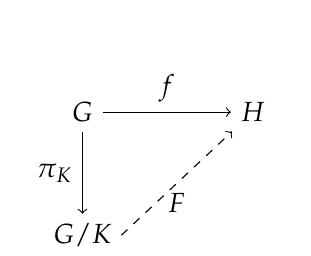
\begin{tikzpicture}
		\matrix (m)
		[
		matrix of math nodes,
		row sep    = 3em,
		column sep = 4em
		]
		{
			G              & H\\
			G/K &             \\
		};
		\path
		(m-1-1) edge [->] node [left] {$\pi_K$} (m-2-1)
		(m-1-1.east |- m-1-2)
		edge [->] node [above] {$f$} (m-1-2)
		(m-2-1.east) edge [->,
		dashed] node [below] {$F$} (m-1-2);
		\end{tikzpicture}
	\end{center}
\end{thm}
\begin{proof}[Proof idea]
	The map is $F: G/K \rightarrow H$ with $F(gK) = f(g)$, it is unique because $\pi_K$ is surjective.
\end{proof}
\begin{cor}
	$G/N \cong \im(f)$.
\end{cor}
\begin{proof}[Proof idea]
	Take $K = N$.
\end{proof}
\begin{cor}
	If $(|G|, |H|) = 1$, then $f$ is trivial (i.e. $\ker(f) = G$).
\end{cor}
\begin{proof}[Proof idea]
	We know that $|G/N|$ divides $|G|$, but also divides $|H|$ since $G/N \cong \im(f)$, this implies $|G/N| = 1$.
\end{proof}
\begin{cor}[Chinese remainder theorem]
	Let $m,n \in \N$ with $(m,n) = 1$, we have $\Z/mn\Z \cong \Z/m\Z \times \Z/n\Z$.
\end{cor}
\begin{proof}[Proof idea]
	Take $f: \Z \rightarrow \Z/m\Z \times \Z/n\Z$ with $f(x) = (x \Mod{m}, x \Mod{n})$ and look at the kernel.
\end{proof}
\begin{thm}[Second isomorphism theorem]
	Let $B < G$ and $N \lhd G$ be subgroups, then $BN/N \cong B/(B \cap N)$.
\end{thm}
\begin{proof}[Proof idea]
	Let $f: BN \rightarrow B/(B \cap N)$ with $f(bn) = b\cdot B\cap N$ and use FIT.
\end{proof}
\begin{thm}[Correspondence theorem]
	Let $f: G \rightarrow H$ be a surjective homomorphism, then $f$ induces a bijection between the subgroups of $G$ containing $\ker(f)$ and the subgroups of $H$. Moreover, let $\ker(f) < G_1 < G_2$, then $G_1 \lhd G_2$ if and only if $f(G_1) \lhd f(G_2)$ giving $G_2/G_1 \cong f(G_2)/f(G_1)$.
\end{thm}
\begin{proof}[Proof idea]
	The first and second part uses definitions, the last part uses the composition $G_2 \rightarrow f(G_2) \rightarrow f(G_2)/f(G_1)$ that has kernel $f^{-1}(f(G_1)) = G_1$, then apply FIT.
\end{proof}
\begin{thm}[Third isomorphism theorem]
	Let $H$ and $K$ be normal subgroups of $G$ such that $H \leq K$, then $(G/H)/(H/K) \cong G/K$.
\end{thm}
\begin{proof}[Proof idea]
	Apply the correspondence theorem with $H = G/N$, $f = \pi_N$, $G_1 = K$ and $G_2 = G$.
\end{proof}

\section{Group Actions}
\begin{lem}[Orbit-Stabilizer formula]
	Let $G$ act on $S$ and $s \in S$, then $|\orb(s)| = \frac{|G|}{|\stab(s)|}$.
\end{lem}
\begin{proof}[Proof idea]
	Let $\phi : G/\stab(s) \rightarrow \orb(s)$, be defined by $\phi(g\stab(s)) = g * s$, show that this is well-defined and that this is an isomorphism.
\end{proof}
\begin{prop}
	Let $G$ act on $S$ and $s, t \in S$ with $t \in \orb(s)$, then $\stab_G(t)$ is conjugate to $\stab_G(s)$.
\end{prop}
\begin{proof}[Proof idea]
	Let $g \in G$ with $g*s = t$ and $h \in \stab(s)$, then $ghg^{-1}*t = t$ and we get $g\stab(s)g^{-1} \subseteq \stab(t)$, we get the other direction similarly. 
\end{proof}
\begin{prop}
	Let $H$ and $K$ be two subgroups of $G$ with finite index, then $H \cap K$ also has finite index in $G$.
\end{prop}
\begin{proof}[Proof idea]
	Let $G$ act diagonally on $G/H \times G/K$, the stabilizer of $(H,K)$ is $H \cap K$, then use the orbit-stabilizer formula.
\end{proof}
\begin{lem}
	A group $G$ acting on $S$ is equivalent to a homomorphism $\phi: G \rightarrow \Sigma_S$, we say that this actions affords the permutation representation $\phi$. Moreover, $\ker(\phi) =\cap_{g\in G} \stab(s)$.
\end{lem}
\begin{proof}[Proof idea]
	For any $g \in G$ and $s \in S$, $\phi(g)(s) = g*s$, this is a homomorphism.
\end{proof}
\begin{thm}[Cayley]
	Every finite group is isomorphic to a subgroup of $S_{|G|}$.
\end{thm}
\begin{proof}[Proof idea]
	Let $G$ act on itself by multiplication, the stabilizers are all trivial, so the permutation representation is injective, the result follows.
\end{proof}
\begin{defn}[Coset representation]
 	Let $H \lhd G$, $G$ acts on $G/H$ affording the homomorphism $\phi : G\rightarrow S_m$ where $m = [G:H]$. $\phi$ is called the coset representation, $\ker(\phi) = \cap_{g\in G}gHg^{-1}$ is the maximal subgroup of $H$ which is normal in $G$.
\end{defn}
\begin{prop}
	Let $G$ be a finite group and $H<G$ of index $p$, where $p$ is the minimal prime dividing the order of $G$, then $H$ is normal in $G$.
\end{prop}
\begin{proof}[Proof idea]
	Consider the coset representation $\phi : G \rightarrow S_p$, we get $p = [G:H]\mid [G:\ker(\phi)]$ and $[G:\ker(\phi)] \mid p!$, leading to $[G:\ker(\phi)] = p$, or $H = K \implies H \lhd G$.
\end{proof}
\begin{thm}[Cauchy-Frobenius Formula]
	Let $G$ act on a set $S$, then the number of ordbits is equal to $\frac{1}{|G|}\sum_{g \in G} \text{\#Fix}(g)$, where $\text{\#Fix}(g)$ denotes the number of fixed points of $G$.
\end{thm}
\begin{proof}[Proof idea]
	Write $T(g,s) = \begin{cases}1 & g*s = s\\0&g*s \neq s\end{cases}$ and observe that $\text{\#Fix}(g) = \sum_{s \in S}T(g,s)$ and $|\stab(s)| = \sum_{g \in G} T(g,s)$. Now expand, rearrange and simplify $\sum_{g \in G} \text{\#Fix}(g)$.
\end{proof}
\begin{cor}
	If $G$ acts transitively on $S$, then there exists a $g \in G$ with no fixed points.
\end{cor}
\begin{proof}[Proof idea]
	Suppose $\text{\#Fix}(g) \geq 1$ for any $g$, use $\text{\#Fix}(e) = |S|$ and CFF to arrive at a contradiction.
\end{proof}
\begin{prop}\label{prop:a3q3}
	Let $G$ act transitively on $S$, $s \in S$ and $K \lhd G$, the number of orbits of $K$ on its action on $S$ is $[G:K\stab_G(s)]$.
\end{prop}
\begin{proof}[Proof idea]
	Observe that $g*K*s = K*s$ if and only if $k^{-1}g \in \stab_G(s)$ if and only if $g \in K\stab_G(s)$. Since the action of $G$ on the $K$ orbits is transitive, $G/(K\stab_G(s))$ is in bijection with the $K$ orbits.
\end{proof}
\section{Symmetric Group}
\begin{lem}
	Two elements $\sigma, \tau \in S_n$ are conjugates if and only if they have the same cycle type.
\end{lem}
\begin{proof}[Proof idea]
	Use the fact that $\tau(i_1\ i_2\dots i_t)\tau^{-1} = (\tau(i_1)\ \tau(i_2)\dots \tau(i_t))$ and find the $\tau$ that works in reverse.
\end{proof}
\begin{cor}
	There are $p(n)$ conjugacy classes in $S_N$, where $p(n)$ denotes the number of partitions of $n$.
\end{cor}
\begin{lem}
	The $S_n$-conjugacy class of an element $\sigma \in A_n$ is a disjoint union of $[S_n : A_n \cent_{S_n}(\sigma)]$ $A_n$-conjugacy classes. In particular, there are two such conjugacy classes if there is an odd permutation commuting with $\sigma$, otherwise there is only one.
\end{lem}
\begin{proof}[Proof idea]
	Apply proposition $\ref{prop:a3q3}$ with $G= S_n$, $K = A_n$ and $S$ being the conjugacy class of $S_n$.
\end{proof}
\begin{lem}
	Let $\sigma \in A_N$, then $\cent_{S_n}(\sigma)$ contains odd permutation unless the disjoint cycle form of $\sigma$ contains only odd cycles of different lengths.
\end{lem}
\begin{lem}
	A normal subgroup $N \lhd G$ is a union of disjoint conjugacy classes.
\end{lem}
\begin{proof}[Proof idea]
	The conjugacy classes are orbits of a group action so they are disjoint, $N$ being normal implies the conjugacy classes of all its elements are contained in $N$.
\end{proof}
\begin{lem}
	The alternating group $A_5$ is simple.
\end{lem}
\begin{proof}[Proof idea]
	Look at the cycle types and the size of each conjugacy class in $A_5$ by observing the conjugacy classes in $S_5$ as well. Conclude that a normal group can only have size 1 or 60.
\end{proof}
\begin{thm}
	The alternating groups $A_n$ are simple for $n \geq 5$.
\end{thm}
\begin{proof}[Proof idea]
	Proof by induction, base case done above. Let $N \lhd A_n$, with $N \neq \{1\}$, show that for any $i$, there is a non-trivial $\rho \in N$ such that $\rho(i) = i$. Now, consider each copy of $A_{n-1}$ that fixes an element $i$, call it $G_i$. Since $G_i$ is simple and $N\cap G_i$ is normal in $G_i$, $N \cap G_i = G_i$, this shows that $N \supseteq \langle G_1, \dots, G_n \rangle = A_n$.
\end{proof}
\begin{prop}
	Suppose that $A_n$ acts transitively on a set of size $m>1$, then $m \geq n$.
\end{prop}
\begin{proof}[Proof idea]
	
\end{proof}
\begin{prop}
	Let $\sigma \neq 1$ be a permutation of $S_n, n \geq 3$, then the conjugacy class of $\sigma$ has more than one element. 
\end{prop}

\section{$p$-groups, Cauchy's and Sylow's theorems}
\begin{lem}[Class equation]
	Let $G$ be a group, then we have the class equation:
	\[|G| = |Z(G)| + \sum_{\text{reps }x \notin Z(G)} \frac{|G|}{|\cent_G(x)|}\]
\end{lem}
\begin{prop}
	If $G$ has an even number of conjugacy classes, then $G$ has even order.
\end{prop}
\begin{proof}[Proof idea]
	Observe that the inverse function $f$ acts on the conjugacy classes and induces a bijection $\conjc(x) \leftrightarrow \conjc(x^{-1})$. Since $f$ fixes $\conjc(1)$, it fixes another one, yielding a bijection on some $\conjc(x_0)$ with $x_0 \neq 1$. If $|G|$ were odd, $|\conjc(x_0)|$ must be odd but since $f^2 = 1$, this implies $f$ fixes a point in $\conjc(x_0)$ which leads to a contradiction. 
\end{proof}
\begin{lem}
	For any $M \in \N$, up to isomorphisms, there are finitely many groups of order at most $M$.
\end{lem}
\begin{proof}[Proof idea]
	Consider the number of possible binary functions.
\end{proof}
\begin{lem}
	Let $q \in \Q_{> 0}$, and $k \in \N$, there are finitely many tuples of positive integers $(n_1, \dots, n_k)$ such that $q = \frac{1}{n_1} + \cdots + \frac{1}{n_k}$.
\end{lem}
\begin{proof}[Proof idea]
	Order the fractions in increasing order, deduce a bound for the last denominator and then use induction on $q-\frac{1}{n_k}$ and a tuple of $k-1$ integers.
\end{proof}
\begin{thm}
	Let $N \in \N$, up to isomorphism, there are finitely many finite groups with $N$ conjugacy classes.
\end{thm}
\begin{proof}[Proof idea]
	Use the last lemma with the class equation.
\end{proof}
\begin{lem}
	Let $G$ be a $p$-group (i.e. $|G| = p^r, r \in \N$), then $Z(G) \neq \{1\}$.
\end{lem}
\begin{proof}[Proof idea]
	Write the class equation, then look at the equation in $\Z/p\Z$.
\end{proof}
\begin{lem}
	Let $G$ be a $p$-group and $H \neq \{1\}$ a normal subgroup, $H \cap Z(G) \neq \{1\}$.
\end{lem}
\begin{proof}[Proof idea]
	Write the class equation for the action of $G$ on $H$ by conjugation, then look at the equation in $\Z/p\Z$.
\end{proof}
\begin{thm}
	Let $G$ be a $p$-group, then the following holds:
	\begin{enumerate}
		\item For any $H \lhd G$, $H \neq G$, there exists $H^{+} \lhd G$ such that $H < H^{+}$ and $[H^+:H] = p$.
		\item For any $H \lhd G$, $H \neq \{1\}$, there exists $H^{-} \lhd G$ such that $H^- < H$ and $[H^-:H] = p$.
	\end{enumerate}
\end{thm}
\begin{proof}[Proof idea]
	\begin{enumerate}
		\item[]
		\item Since $G/H$ is a $p$-group, there is a non-trivial $x \in Z(G/H)$, the order of $x$ is a power of $p$, so you can get $y$ of order $p$. Let $K = \langle y \rangle \lhd G/H$, we then use the quotient map and the correspondence theorem to lift $K$ to $H^+$. 
		\item Use induction, case $|G| = p$ is clear. Choose an element $x \in H \cap Z(G)$ of order $p$. Let $K = \langle x \rangle \lhd G$, note that $K \subseteq H$. If $H = K$, take $H^- = \{1\}$. Otherwise, apply induction on $G/K$ to find $(H/K)^{-}$ and use the correspondence theorem to lift it to $H^-$.
	\end{enumerate}
	
\end{proof}
\begin{lem}
	Let $G$ be any group and $H \subset Z(G)$ such that $G/H$ is cyclic, then $G$ is abelian.
\end{lem}
\begin{proof}[Proof idea]
	Let $g \in G$ be such that $gH$ generates $G/H$. This implies that every element is of the form $g^ih$, show that these elements commute.
\end{proof}
\begin{defn}[Frattini subgroup]
	The Frattini subgroup of a $p$-group $G$ , denoted $\Phi(G)$, is the intersection of all the maximal subgroups of $G$.
\end{defn}
\begin{prop}\label{prop:fratt}
	Let $G$ be a $p$-group, $\Phi(G) \lhd G$ is a non-trivial abelian group where every non-zero element is of order $p$. It is the largest quotient with this property. Also, $\Phi(G) = G^pG'$.
\end{prop}
\begin{proof}[Proof idea]
	Conjugation takes maximal subgroups to maximal subgroups so $\Phi(G)$ is normal. The index of a maximal subgroup $H$ forces $G/H$ to be abelian, so $H \supseteq G'$, implying $\Phi(G) \supseteq G'$ so $G/\Phi(G)$ is also abelian. Also, $gH$ has order $p$ so $g^p \in H$ and $H \supseteq G^p$ implying $\Phi(G) \supseteq G^p$. We get that $\Phi(G) \supseteq G^pG'$ and every non-trivial element has order $p$, this is true for any $N \lhd G$ with $G/N$ abelian and elements killed by $p$. Then show $\Phi(G) \subseteq G^pG'$ by passing to a vector space over $\F_p$.
\end{proof}
\begin{lem}
	Let $A$ be a finite abelian group with a prime $p \mid |A|$, $A$ has an element of order $p$.
\end{lem}
\begin{proof}[Proof idea]
	We use induction, case $|A| = p$ is clear. Let $N$ be a maximal subgroup of $A$, it is normal because $A$ is abelian. If $p$ divides $|N|$ use induction. Otherwise, take $x \in A \setminus N$ and let $B = \langle x \rangle$, show that $p \mid |B|$, so we can find an element of order $p$.
\end{proof}
\begin{prop}
	Let $G$ be a non-commutative $p$-group and $H$ be a normal subgroup such that $G/H$ is abelian and $|H| = p$, then $H = G'$. If every element of $G/H$ has order $p$, then $H = \Phi(G)$.
\end{prop}
\begin{proof}[Proof idea]
	By the definition of $G'$, we have $G' \subseteq H$, but $G' \neq \{1\}$, so we must have $G' = H$. The second statement follows from proposition \ref{prop:fratt}.
\end{proof}
\begin{prop}
	Let $G$ be a group of order $p^rm$ where $p$ is prime and $(p,m) = 1$, there exists a subgroup of order $p^r$.
\end{prop}
\begin{proof}[Proof idea]
	We use induction, the case $|G| = p$ is clear. If $p \mid |Z(G)|$, then take $N = \langle x \rangle \lhd G$, where $x$ is of order $p$. Consider $G/N$, its order is $p^{r-1}m$, we can use induction and the correspondence theorem to lift a group of order $p^r$.
	
	In the case where $p \nmid |Z(G)|$. Consider the class equation modulo $p$, and find that $\cent_G(x)$ is a proper subgroup of order divisible by $p^r$ so we can use induction.
\end{proof}
\begin{cor}
	Let $p_1^{a_1}\cdots p_k^{a_k}$ be the prime factorization of $|G|$ and $P_i$ be a subgroup of size $p_i^{a_i}$, then $G = \langle P_1, \dots, P_k \rangle$.
\end{cor}
\begin{proof}[Proof idea]
	The order of $\langle P_1, \dots, P_k \rangle$ is divisible by the order of the group.
\end{proof}
\begin{cor}[Cauchy's theorem]
	Let $G$ be finite with $p \mid |G|$, then $G$ has an element of order $p$.
\end{cor}
\begin{proof}[Proof idea]
	We find a subgroup of order $p^r$, find an element of order $p^b$ and then transform it to an element of order $p$.
\end{proof}
\begin{lem}
	Let $P$ be a maximal $p$-subgroup of $G$ and $Q$ be any $q$-subgroup of $G$, where $q$ is a different prime. $Q \cap P = Q \cap N_G(P)$.
\end{lem}
\begin{proof}[Proof idea]
	Since $P \subseteq N_G(P)$, we have $Q \cap P \subseteq Q \cap N_G(P) =: H$. For the other direction, see that $HP$ is a $p$-subgroup of $N_G(P)$ but it must be $P$ since $P$ is maximal. This yields $H \subseteq P$ and the result follows.
\end{proof}
\begin{thm}[Sylow]
	Let $G$ be a group of order $p^rm$ where $p$ is prime and $(p,m) = 1$, the following holds:
	\begin{enumerate}
		\item Every maximal $p$-subgroup has order $p^r$ (they are called $p$-Sylow subgroups).
		\item All $p$-Sylow subgroups are conjugate to each other.
		\item Let $n_p = |\syl_p(G)|$, then $n_p \equiv 1 \Mod{p}$ and $n_p \mid m$.
	\end{enumerate}
\end{thm}
\begin{proof}[Proof idea]
	Let $S = \{P_1, \dots, P_a\}$ be the set of conjugates of some $p$-Sylow $P$. Let $Q$, any $p$-subgroup, act by conjugation on $S$, the size of $\orb(P_i)$ is $\frac{|Q|}{|\stab_Q(P_i)|} = \frac{|Q|}{|Q \cap P_i|}$. We see that the sizes are a power of $p$ unless $Q \subseteq P_i$, in that case, the size is one.
	
	If we take $Q = P_1$, we know that only the orbit of $P_1$ has size 1 because $P_1$ is maximal. Hence, $S$ being the disjoin union of orbits has size congruent to 1 modulo $p$. Suppose towards a contradiction that $Q$ is a maximal subgroup not in $S$ and let it act on $S$. We get that all the orbits are congruent to 0 modulo $p$, contradicting our previous statement. Lastly, if we use the orbit stabilizer formula on the action of $G$ by conjugation on the set of maximal subgroups, we get $a = \frac{|G|}{|N_G(P)|}$, so $a$ divides $|G|$. 
\end{proof}
\begin{lem}
	Let $G$ be finite, $p \neq q$ be two primes dividing $|G|$ and $P \in \syl_p(G), Q \in \syl_q(G)$, then $P \cap Q = \{1\}$.
\end{lem}
\begin{proof}[Proof idea]
	The size of $P \cap Q$ divides $|P|$ and $|Q|$, since $(p,q) = 1$, we must have $|P \cap Q| = 1$.
\end{proof}
\begin{lem}
	Let $G$ be any group and $A,B \lhd G$, then for any $a \in A$ and $b \in B$, $ab = ba$.
\end{lem}
\begin{proof}[Proof idea]
	Note that $aba^{-1}b^{-1}$ is in both $A$ and $B$ so it must be 1, the result follows.
\end{proof}
\begin{prop}
	Let$p_1^{a_1}\cdots p_k^{a_k}$ be the prime factorization of $|G|$ and $P_i$ be a $p_i$-Sylow subgroup. $G = P_1 \times \cdots \times P_k$ if and only if for any $i$, $P_i \lhd G$.
\end{prop}
\begin{proof}[Proof idea]
	Suppose all the $P_i$ are normal, then take $f: P_1 \times \cdots \times P_k \rightarrow G$ be defined by $f(x_1, \dots, x_k) = x_1x_2\cdots x_k$. Since $P_i$ and $P_j$ commute for $i\neq j$, $f$ is a homomorphism, then show it is bijective.
\end{proof}
\begin{prop}
	Let $G$ be finite, $H \lhd G$ and $P$ be a $p$-Sylow subgroup of $G$. $P \cap H$ is a maximal $p$-subgroup and $HP/H$ is a $p$-Sylow subgroup of $G/H$.
\end{prop}
\begin{proof}[Proof idea]
	Show that $|Q \cap H| = |P \cap H|$ for any $p$-Sylow $Q$ of $G$. Since a $p$-Sylow of $H$ is contained in a $p$-Sylow of $G$, we see by cardinality that $H\cap P$ must be a $p$-Sylow of $H$. For the second part, calculate the size of $HP/H$ and $G/H$. 
\end{proof}
\begin{defn}[Nilpotent groups]
	A nilpotent group only has normal Sylow subgroups. Equivalently, for any prime $p$ dividing the order of the group, there is a unique $p$-Sylow subgroup.
\end{defn}
\section{Composition Series and Solvable Groups}
\begin{defn}
	A normal series for $G$ is a series of subgroups $G = G_0 \rhd \cdots \rhd G_n = \{1\}$ (it is usually strictly descending, namely $G_i \neq G_j$ for $i \neq j$).
\end{defn}
\begin{defn}
	A composition series for $G$ is a normal series such that $G_{i-1}/G_i$ is non-trivial and simple for all $i \in \{1,\dots, n\}$. The quotients are called the composition factors, they are considered up to isomorphism but with multiplicity.
\end{defn}
\begin{defn}
	A group $G$ is called solvable if it has a normal series in which all the composition factors are abelian.
\end{defn}
\begin{lem}
	Any strictly descending normal series can be refined to a composition series. Moreover, if the composition factors are abelian, the refinement has composition factors isomorphic to $\Z/p\Z$ for some prime $p$.
\end{lem}
\begin{proof}[Proof idea]
	Note that the quotients are non trivial and that $|G|$ is the product of the orders of the quotients. Hence, a strictly descending normal series has bounded length. Assume that the series is not a composition series, take $G_{i-1}/G_i$ that is not simple and take a non-trivial normal subgroup $H'$, lift it to $G_{i-1}$ and extend the series to $\cdots G_{i-1} \rhd H \rhd G_i \cdots$, the first part follows. For the second part, note that our construction still has abelian quotients. Also, finite abelian simple groups are isomorphic to $\Z/p\Z$. 
\end{proof}
\begin{cor}
	A group $G$ is solvable if and only if it has a composition series with composition factors being cyclic groups of prime order.
\end{cor}
\begin{thm}[Jordan-H\"older]
	Let $G$ be finite, any two composition series for $G$ have the same composition factors (considered with multiplicity).
\end{thm}
\begin{exmps}
	Any abelian group is solvable, $p$-groups are solvable, groups of order $pq$ are solvable, groups of order $p^2q$ are solvable, groups of order $pqr$ are solvable and the product of solvable groups are solvable.
\end{exmps}
\begin{prop}
	Let $G$ be solvable and $K <G$, $K$ is solvable.
\end{prop}
\begin{proof}[Proof idea]
	Intersect $K$ with the groups in the normal series with abelian quotients for $G$, we get a normal series with abelian quotients but for $K$.
\end{proof}
\begin{defn}
	A short exact sequence is a sequence of group and homomorphism $1 \rightarrow G_1 \stackrel{f}{\rightarrow} G_2 \stackrel{g}{\rightarrow} G_3 \rightarrow 1$ with $f$ injective, $g$ surjective and $\im(f) = \ker(g)$.
\end{defn}
\begin{prop}
	Let $1 \rightarrow K \rightarrow G \rightarrow H \rightarrow 1$ be a short exact sequence, $G$ is solvable if and only if $K$ and $H$ are solvable.
\end{prop}
\begin{proof}[Proof idea]
	Assume that $G$ is solvable, then $f(K)$ is solvable (hence $K$ as well). If $G_i$ are the groups in the normal series for $G$, let $H_i= g(G_i)$ be the ones for $H$, then show that this is a normal series with abelian factors.
	
	Assume $K$ and $H$ are solvable. Let $J_i = g^{-1}(H_i)$ and $J_i = f(K_{i-n})$ for the rest, $J_i$ is a normal series with abelian quotients.
\end{proof}
\begin{thm}
	Every group of order less than 60 is solvable.
\end{thm}
\begin{thm}[Burnside]
	Every group of order $p^aq^b$ is solvable.
\end{thm}
\begin{thm}[Feit-Thompson]
	Every finite group of odd order is solvable.
\end{thm}

\section{Finitely Generated Abelian Groups and Semidirect Products}
\begin{defn}
	A group $G$ is called finitely many generated if there are elements $g_1, \dots, g_n$ in $G$ such that $G = \langle g_1, \cdots, g_n\rangle$.
\end{defn}
\begin{lem}
	An abelian group $G$ is finitely generated if for some positive integer $n$, there is a surjective homomorphism from $\Z^n$ to $G$.
\end{lem}
\begin{thm}[Structure theorem]
	Let $G$ be a finitely generated abelian group, then there exists unique $r \in \N$ and $n_1, \dots, n_t \in \N_{> 1}$ such that $G \cong \Z^r \times \Z/n_1\Z \times \cdots \times \Z/n_t\Z$.
\end{thm}
\begin{defn}
	Let $G$ be a group and $B$ and $N$ be subgroups of $G$ such that $G = NB$, $N\cap B = \{1\}$ and $N \lhd G$. We say that $G$ is a semidirect product of $N$ and $B$. Also, if $N$ and $B$ are groups and $\phi: B \rightarrow \aut(N)$ is a group homomorphism, we define $N \rtimes_{\phi} B$ to be the semidirect product of $N$ and $B$ relative to $\phi$. It is the group $N \times B$ with the following operation:
	\[ (n_1,b_1) \cdot (n_2,b_2) = (n_1 \phi(b_1)(n_2), b_1b_2) \]
\end{defn}
\begin{prop}
	$N  \rtimes_{\phi} B \cong N \times B$ if and only if $\phi$ is trivial.
\end{prop}
\begin{proof}[Proof idea]
	Use the definitions.
\end{proof}
\begin{prop}
	$N \rtimes_{\phi} B$ is abelian if and only if both $N$ and $B$ are abelian and $\phi$ is trivial.
\end{prop}
\begin{proof}[Proof idea]
	Use the definitions.
\end{proof}
\begin{prop}\label{prop:iso}
	Let $N$ and $B$ be groups and $\phi$ and $\psi$ be homomorphisms $B \rightarrow \aut(N)$, then $N \rtimes_{\phi} B \cong N \rtimes_{\psi} B$ if and only if there exists automorphisms $f \in \aut(N)$ and $g \in \aut(B)$ such that $\forall b \in B, \psi(b) = f \circ \phi(g(b)) \circ f^{-1}$. The isomorphism between the two semidirect products is $(n,b) \mapsto (f(n), g^{-1}(b))$.
\end{prop}
\begin{proof}[Proof idea]
	Just verify that the map seen is an isomorphism.
\end{proof}
\begin{lem}
	Let $n \in \N$, $\aut(\Z/n\Z) \cong (\Z/n\Z)^{\times}$.
\end{lem}
\begin{proof}[Proof idea]
	For any $a \in \Z/n\Z$ such that $(a,n) = 1$, show that $f_a(x) = ax$ is in $\aut(\Z/n\Z)$, then show that $a \mapsto f_a$ is an isomorphism. 
\end{proof}
\begin{prop}
	If $p \mid (q-1)$, there is a unique non-abelian group of order $pq$.
\end{prop}
\begin{proof}[Proof idea]
	We know that any $q$-Sylow $Q$ is normal. Let $P$ be any $p$-Sylow, $G$ is a semidirect product of $Q$ and $P$. There is a non-abelian semidirect product when $\phi$ maps $1$ to $a \mapsto ha$, where $h$ is an element of order $p$ of $(\Z/q\Z)^{\times}$. It is clear that any other homomorphism that works will just have a different $h$, but then we can transform it as in proposition \ref{prop:iso} to get the isomorphism.
\end{proof}

\section{Complex Representation of Finite Groups}
\begin{defn}[Representation]
	Let $G$ be a finite group, $V$ be a finite dimensional vector space over $\mathbb{C}$ and $\rho: G \rightarrow \aut(V)$ be a group homomorphism, $(\rho, V)$ is called a finite representation of $G$.
\end{defn}
\begin{defn}[Morphism of representation]
	Let $(\rho, V)$ and $(\tau, W)$ be representations of a finite group $G$, a linear map $T: V_1 \rightarrow V_2$ is called a morphism of $\rho_1$ to $\rho_2$ if for any $g \in G$, $\rho_2(g) \circ T = T \circ \rho_1(g)$. We will denote $\homm_G(V_1, V_2)$ to be the subspace of $\homm(V_1, V_2)$ with linear maps satisfying this property.
\end{defn}
\begin{defn}[Character group]
	For a group $G$, the character group of $G$, denoted $G^*$, is the set of group homomorphisms from $G$ to $\mathbb{C}^{\times}$.
\end{defn}
\begin{prop}
	The following are properties of the character group.
	\begin{enumerate}
		\item $(H \times G)^{*} \cong H^* \times G^*$.
		\item $(\Z/n\Z)^* \cong \Z/n\Z$.
		\item If $G$ is finite and abelian, $G^* \cong G$.
		\item For a general group $G$, $G^* = (G/G')^*$.
	\end{enumerate}
\end{prop}
\begin{proof}[Proof idea]
	\begin{enumerate}
		\item Define the map $\phi : (H \times G)^* \rightarrow H^* \times G^*$ with $f \mapsto (f(\cdot, 1), f(1, \cdot))$. Show that it is an isomorphism.
		\item Observe that $f \in (\Z/n\Z)^*$ is only defined by where it sends the generator, and it must send it to a generator of the group of $n$th roots of unity (this group is isomorphic to $\Z/n\Z$).
		\item Use the structure theorem and the two previous points.
		\item Show that if $f \in G^*$, then $f([x,y]) = 1$ and so $G' \subseteq \ker(f)$, then the result follows from the first isomorphism theorem.
	\end{enumerate}
\end{proof}
\begin{thm}
	Let $(\rho, V)$ be a representation of $G$, there exists a inner product that is $G$-invariant (i.e. for all $v,w \in V$, $\inp{\rho(g)v}{\rho(g) w} = \inp{v}{w}$).
\end{thm}
\begin{proof}[Proof idea]
	Take any inner product $(\cdot, \cdot)$ and let $\inp{u}{v} = \frac{1}{|G|}\sum_{g \in G}(\rho(g)u, \rho(g)v)$, verify that $\inp{\cdot}{\cdot}$ is $G$-invariant.
\end{proof}
\begin{thm}
	Any representation decomposes as a sum of irreducible representations.
\end{thm}
\begin{proof}[Proof idea]
	Argue by induction. If $U$ is a subrepresentation, then $U^{\perp}$ (w.r.t. a $G$-invariant inner product) is also a subrepresentation.
\end{proof}
\begin{thm}
	Let $G$ be an abelian group, every representation of $G$ decomposes into a direct sum of $1$-dimensional representations.
\end{thm}
\begin{proof}[Proof idea]
	First prove that $\rho(g)$ is diagonalizable. Then use the fact that commuting diagonalizable linear operator are simultaneously diagonalizable.
\end{proof}
\begin{lem}[Schur]
	Let $(\rho, V)$ and $(\tau, W)$ be irreducible representations of $G$, we have the following: \[\homm_G(V,W) \cong \begin{cases}0 & \rho \not\cong \tau\\ \mathbb{C} & \rho \cong \tau \end{cases}\]
\end{lem}
\begin{proof}[Proof idea]
	Note that if $T \in \homm_G(V,W)$, $\ker(T)$ and $\im(T)$ are subrepresentations, this implies $T$ is either trivial or an isomorphism. Now, look at an eigenspace of $T$ and show that it must be equal to the whole vector space.
\end{proof}
\begin{defn}
	Let $(\rho, V)$ and $(\tau, W)$ be representations of $G$, $\sigma : G \rightarrow \aut(\homm(V,W))$ is a new representation with $\sigma(g) T = \tau(g) \circ T \circ \rho(g^{-1})$.
\end{defn}
\begin{thm}
	 We get that for any $g \in G$, $\chi_{\sigma}(g) = \overline{\chi_{\rho}(g)}\chi_{\tau}(g)$.
\end{thm}
\begin{proof}[Proof idea]
	No need to learn it.
\end{proof}
\begin{defn}
	Let $(\rho, V)$ be a representation of $G$, define the projection operator as $\pi_{\rho} : V \rightarrow V$ with $\pi_{\rho} = \frac{1}{|G|} \sum_{g \in G} \rho(g)$.
\end{defn}
\begin{thm}
	If $\rho = \rho_1^{a_1} \oplus \cdots \oplus \rho_t^{a_t}$ where $\rho_1$ is the trivial representation, then $$\pi_{\rho} = \text{Id}_{V_1^{a_1}} \oplus 0 \oplus \cdots \oplus 0$$
	From this, we get the following:
	\[ a_1 = \text{Tr}(\pi_{\rho}) = \frac{1}{|G|}\sum_{g \in G} \chi_{\rho}(g) = \inp{\chi_{\rho}}{\chi_1} \]
\end{thm}
\begin{proof}[Proof idea]
	Note that $V^G = (V_1^{a_1})^G \oplus \cdots \oplus (V_1^{a_t})^G$ and that except for $i = 1$, $(V_i^{a_i})^G = \{0\}$ because it is a subrepresentation. The result follows.
\end{proof}
\begin{thm}
	The characters of irreducible representations are orthogonal with respect to the $G$-invariant inner product.
\end{thm}
\begin{proof}[Proof idea]
	Use $\dim(\homm(V,W)^G) = \frac{1}{|G|}\sum_{g \in G} \chi_{\sigma}(g) = \inp{\chi_{\rho}}{\chi_{\tau}}$. Then use Schur's lemma.
\end{proof}
\begin{prop}
	Here are some consequences of the last theorem.
	\begin{enumerate}
		\item A representation $\rho$ decomposes into an irreducible representation: $\rho = \rho_1^{a_1} \oplus \cdots \oplus \rho_t^{a_t}$.
		\item $a_i = \inp{\chi_{\rho}}{\chi_{\rho_i}}$.
		\item $\chi_{\rho}$ determines $\rho$ up to isomorphism.
		\item $\rho^{\text{reg}} = \rho_1^{\dim(\rho_1)} \oplus \cdots \oplus \rho_t^{\dim(\rho_t)}$.
		\item $\rho$ is irreducible if and only if $\norm{\chi_{\rho}} = 1$.
		\item There exists finitely many irreducible characters (hence representations).
	\end{enumerate}
\end{prop}
\begin{proof}[Proof idea]
	\begin{enumerate}
		\item[]
		\item Done above.
		\item Follows from orthogonality of the irreducible characters.
		\item Follows from the last part.
		\item Follows from the fact that $\chi_{\text{reg}}$ is 0 everywhere but on the identity.
		\item Follows from orthonormality of the irreducible characters.
		\item Since they are orthonormal, they can be bigger than the dimension of $\text{Class}(G)$.
	\end{enumerate}
\end{proof}
\begin{defn}
	We define a more general operator. Let $\alpha \in \text{Class}(G)$, we define the operator $A_{\rho} = \sum_{g \in G} \alpha(g)\rho(g)$.
\end{defn}
\begin{lem}
	For two representations $\rho$ and $\tau$ of $G$, $A_{\rho \oplus \tau} = A_{\rho} \oplus A_{\tau}$.
\end{lem}
\begin{proof}[Proof idea]
	Use the definitions.
\end{proof}
\begin{thm}
	Let $\chi_{\rho_1}, \dots, \chi_{\rho_t}$ be the characters of all the irreducible representations of $G$, they form an orthonormal basis of $\text{Class}(G)$, in particular, $t = h(G)$.
\end{thm}
\begin{proof}[Proof idea]
	Let $\beta \in \text{Class}(G)$ be a function orthogonal to all irreducible characters. Let $\alpha = \overline{\beta}$ and for an irreducible representation $\rho_i$, show that $A_{\rho_i} \equiv 0$. Using the last lemma, we get $A_{\rho^{\text{reg}}} \equiv 0$, which is equivalent to $\alpha = \overline{\beta} \equiv 0$.
\end{proof}
\begin{prop}
	Let $g, h \in G$ and $\{\chi_i \mid i \in \{1,\dots, h(G)\}\}$ be the irreducible representations of $G$, then:\[ \sum_{i=1}^{h(G)} \chi_i(g)\overline{\chi_i(h)} = \begin{cases}|\cent_G(g)| & \mbox{if $g$ and $h$ are conjugate}\\0& \mbox{otherwise}\end{cases} \]
\end{prop}
\begin{proof}[Proof idea]
	Let $g_i$ be the representative for the conjugacy classes and $c_i = |\conjc(g_i)|$, also let $T$ be the character table (i.e. $(T)_{ij} = \chi_i(g_j)$) and $D = \text{diag}\bra{\frac{|c_1|}{n}, \dots, \frac{|c_{h(G)}|}{n}}$. The row orthogonality condition says that $TDT^* = I_{h(G)}$, implying that $T^{-1} = DT^*$. We obtain $T^*T = D^{-1} \text{diag}\bra{\frac{n}{|c_1|}, \dots, \frac{n}{|c_{h(G)}|}}$, showing the result since $\frac{|G|}{|\conjc(g)|} = |\cent_G(g)|$.
\end{proof}
\begin{prop}
	For $n \geq 4$, the representation $\rho^{st,0}$ of $A_n$ is irreducible.
\end{prop}
\begin{proof}[Proof idea]
	Recall that $\chi = \chi_1 + \chi_0$ where $\chi$ is the standard representation, $\chi_1$ is the trivial one and $\chi_0 = \chi_{\rho^{st,0}}$. We will use $\norm{\chi}^2 = \norm{\chi_1}^2 + \inp{\chi_1}{\chi_0} + \inp{\chi_0}{\chi_1} + \norm{\chi_0}^2$. Show that $\norm{\chi}^2 = 2$, let $A_n$ act diagonally on $\{1,\dots, n\}^2$, show that there are two orbits, then use CFF with the fact that $\text{\#Fix}(\sigma) = \chi(\sigma)$. Now, show that $\inp{\chi_1}{\chi_0} = \inp{\chi_0}{\chi_1} = 0$ and since $\chi_1$ is irreducible, the result follows.
\end{proof}
\begin{prop}
	Let $z \in Z(G)$ and $V$ be an irreducible representation of $G$, then $z$ acts on $V$ as a multiple of the identity.
\end{prop}
\begin{proof}[Proof idea]
	Let $V_{\lambda}$ be an eigenspace of $\rho(z)$, show that $V_{\lambda}$ is a non-trivial subrepresentation, hence equal to $V$.
\end{proof}
\end{document}